\documentclass[UTF8]{ctexart}
\usepackage{graphicx}
\usepackage{geometry}
\usepackage{fancyhdr}
\geometry{papersize={21.0cm,29.7cm}}
\geometry{left=3.18cm,right=2.54cm,top=2.54cm,bottom=3.18cm}
\title{涉众分析文档}
\author{吴康康}
\date{2015年10月14日}
\pagestyle{fancy}
\lhead{}
\chead{涉众分析文档}
\rhead{大学生锻炼助手}
\lfoot{}
\cfoot{\thepage}
\rfoot{}
\renewcommand{\headrulewidth}{0.4pt}
\renewcommand{\headwidth}{\textwidth}
\renewcommand{\footrulewidth}{0pt}

\begin{document}
\maketitle
\section{涉众识别过程}
\subsection{识别涉众类别}
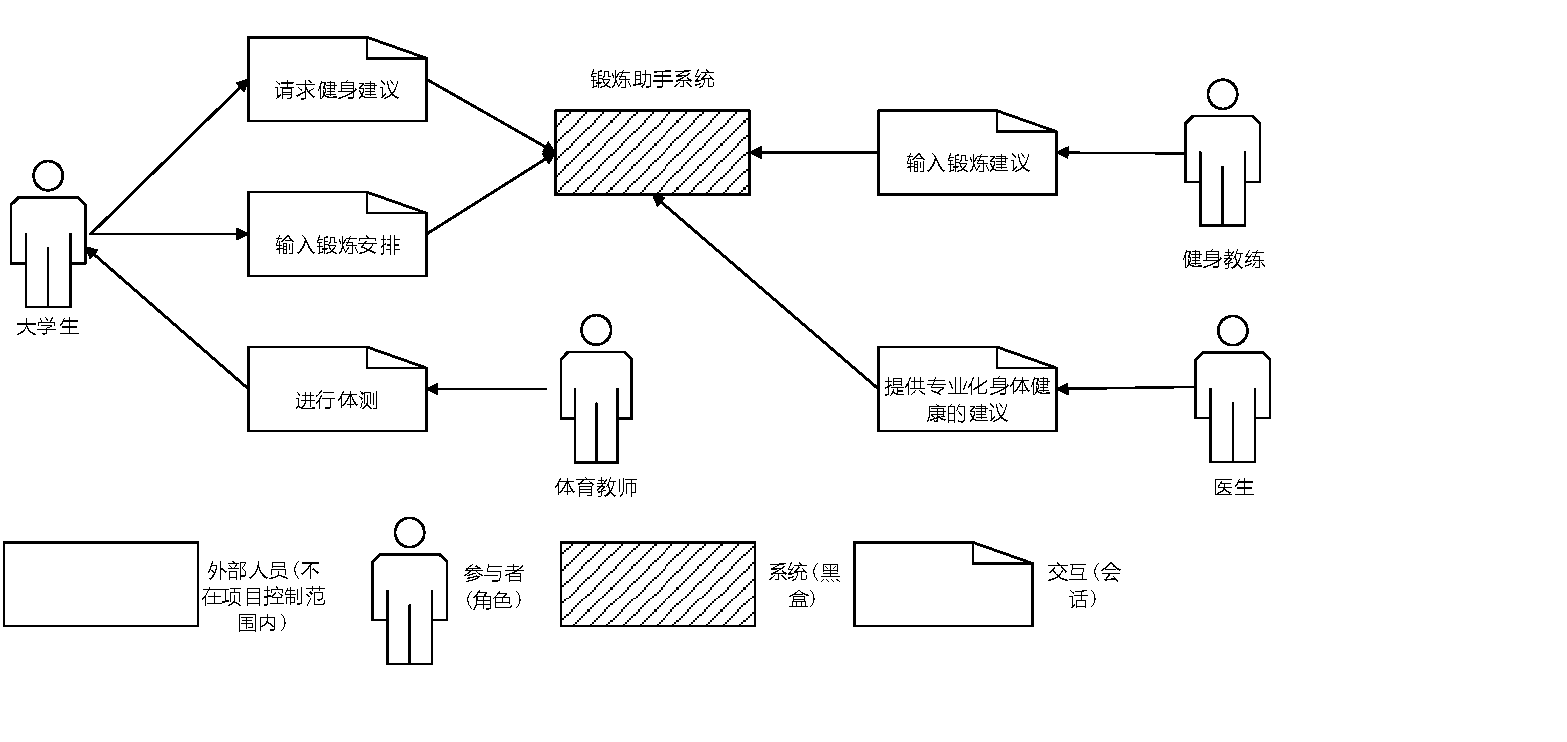
\includegraphics[scale=0.60]{figure.pdf}
\section{涉众描述与优先级}
\centering
\begin{tabular}{|p{3cm}|p{1.8cm}|p{1.2cm}|p{2.5cm}|p{2cm}|p{2cm}|}
 \hline
涉众& 特点& 优先级& 主要目标& 态度& 主要关注点\\
 \hline
体质较差、缺少锻炼的大学生 & 学业忙,时间紧 & 高 & 增强体质,提高体测成绩,扩大交际圈 & 强烈要求提高成绩 & 成绩 \\
 \hline
体质较好、热爱运动的大学生 & 学业忙,时间紧 & 中 & 扩大交际圈 &希望交到朋友 & 社交 \\
  \hline
医生 & 工作忙,不一定能及时回答 & 中 & 提供专业化身体健康的建议 & 平时工作就很忙,基本无所谓 & 身体素质 \\
   \hline
健身教练 & 不便于对计划采纳者进行督促与质量检测 & 中 & 提供专业化锻炼计划的建议 & 希望帮助他人 & 运动机能 \\
      \hline
\end{tabular}
\section{共赢分析}
\end{document}
